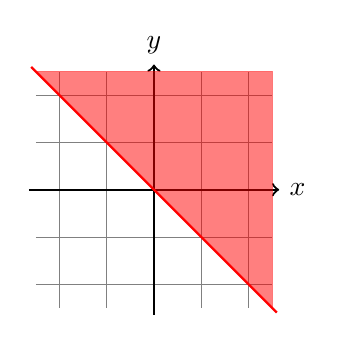
\begin{tikzpicture}[scale=.3]
	\def\xone{-5}
	\def\xtwo{5}
	\def\yone{-5}
	\def\ytwo{5}

% grid
  \draw[step=2cm,help lines] (\xone,\yone) grid (\xtwo,\ytwo);
  \draw[thick,->] (\xone-.3, 0) -- (\xtwo+.3, 0) node[right] {$x$};
  \draw[thick,->] (0, \yone-.3) -- (0, \ytwo+.3) node[above] {$y$};

% def domain
  \filldraw[red,opacity=.5] (\xone,\ytwo) -- (\xtwo,\ytwo) -- (\xtwo,\yone);
  \draw[red,thick] (\xone-.2,\ytwo+.2) -- (\xtwo+.2,\yone-.2);
  \node[] at (\xtwo/2,\ytwo/2) {$\D$};
\end{tikzpicture}
